\documentclass[UTF8,AutoFakeBold,AutoFakeSlant,zihao=-4]{ctexart}
\usepackage[a4paper,left=2.4cm,right=2.4cm,top=2.6cm,bottom=2.38cm,includeheadfoot]{geometry}   % 设置页面大小
\usepackage{fontspec} % 字体
\usepackage{setspace} % 设置行距
\usepackage{graphicx} % 图片
\usepackage{fancyhdr} % 页眉页脚
\usepackage{pdfpages} % 插入 PDF
\usepackage{setspace} % 设置行距
\usepackage{booktabs} % 表格
\usepackage{multirow} % 表格
\usepackage{caption} % 图片和表格的 caption
\usepackage{subcaption} 
\usepackage{float} 
\usepackage{listings}
\usepackage{color}
\usepackage[colorlinks,linkcolor=blue]{hyperref}

\definecolor{dkgreen}{rgb}{0,0.6,0}
\definecolor{gray}{rgb}{0.5,0.5,0.5}
\definecolor{mauve}{rgb}{0.58,0,0.82}

\lstset{frame=tb,
  language=Python,
  aboveskip=3mm,
  belowskip=3mm,
  showstringspaces=false,
  columns=flexible,
  basicstyle={\small\ttfamily},
  numbers=none,
  numberstyle=\tiny\color{gray},
  keywordstyle=\color{blue},
  commentstyle=\color{dkgreen},
  stringstyle=\color{mauve},
  breaklines=true,
  breakatwhitespace=true,
  tabsize=3
}


\newcommand{\coursename}{《Python程序设计》}
\newcommand{\coursenumber}{U08M11077}
\newcommand{\proname}{2048小游戏开发}
\newcommand{\members}{路人甲~路人乙~路人丙~路人丁}
\newcommand{\phone}{123~1234~1234}
\newcommand{\protime}{2022年12月}

% 定义 caption 字体为楷体
\DeclareCaptionFont{kaiticaption}{\kaishu \normalsize}

% 设置图片的 caption 格式
\renewcommand{\thefigure}{\thesection-\arabic{figure}}
\captionsetup[figure]{font=small,labelsep=space,skip=10bp,labelfont=bf,font=kaiticaption}

% 设置表格的 caption 格式
\renewcommand{\thetable}{\thesection-\arabic{table}}
\captionsetup[table]{font=small,labelsep=space,skip=10bp,labelfont=bf,font=kaiticaption}

% 定义一个概念
\newtheorem{definition}{概念}[section]

% 输出大写数字日期
\CTEXoptions[today=big]


\setromanfont{Times New Roman}



% 设置文档标题深度
\setcounter{tocdepth}{3}
\setcounter{secnumdepth}{3}

%%
% 设置一级标题、二级标题格式
% 一级标题:小三,宋体,加粗,段前段后各半行
\ctexset{section={
  format={\raggedright \bfseries \songti \zihao{-3}},
  beforeskip = 24bp plus 1ex minus .2ex,
  afterskip = 24bp plus .2ex,
  fixskip = true,
  name = {,.}
  }
}
% 二级标题:小四,宋体,加粗,段前段后各半行
\ctexset{subsection={
  format = {\bfseries \songti \raggedright \zihao{4}},
  beforeskip =24bp plus 1ex minus .2ex,
  afterskip = 24bp plus .2ex,
  fixskip = true,
  }
}

%%
% 文档开始
\begin{document}

% 报告封面
\topskip=0pt

\begin{titlepage}
  \vspace*{20mm}
  \centering
  \hspace{0mm}\heiti\fontsize{30pt}{30pt}\selectfont{西北工业大学}

  \vspace{13mm}

  \hspace{0mm}\heiti\fontsize{20pt}{20pt}\selectfont{课程设计(大作业)报告}

  \vspace{40mm}

  \flushleft
  \begin{spacing}{2.2}


    \hspace{36mm}\songti\fontsize{16pt}{16pt}\selectfont{\textbf{课程名称:}\underline{\makebox[72mm][c]{\coursename}}}

    \hspace{36mm}\songti\fontsize{16pt}{16pt}\selectfont{\textbf{课程编号:}\underline{\makebox[72mm][c]{\coursenumber}}}

    \hspace{36mm}\songti\fontsize{16pt}{16pt}\selectfont{\textbf{设计题目:}\underline{\makebox[72mm][c]{\proname}}}

    \hspace{36mm}\songti\fontsize{16pt}{16pt}\selectfont{\textbf{组员名单:}\underline{\makebox[72mm][c]{\members}}}

    \hspace{36mm}\songti\fontsize{16pt}{16pt}\selectfont{\textbf{联系方式:}\underline{\makebox[72mm][c]{\phone}}}

    \hspace{36mm}\songti\fontsize{16pt}{16pt}\selectfont{\textbf{设计时间:}\underline{\makebox[72mm][c]{\protime}}}
  \end{spacing}

  \vspace{47mm}


\end{titlepage}



%%插入一页目录
\newpage
\tableofcontents


% 正文开始
\pagestyle{fancy}
% 正文从第一页开始计算页码
\setcounter{page}{1}
% 页眉和页脚(页码)的格式设定
\fancyhf{}
\fancyhead[R]{\fontsize{10.5pt}{10.5pt}\selectfont{西北工业大学课程设计(大作业)报告}}
\fancyfoot[R]{\fontsize{9pt}{9pt}\selectfont{\thepage}}
\renewcommand{\headrulewidth}{1pt}
\renewcommand{\footrulewidth}{0pt}

% 正文 22 磅的行距,段前段后间距为 0
\setlength{\parskip}{0em}
\renewcommand{\baselinestretch}{1.53}
% 正文首行悬挂 1.02cm
\setlength{\parindent}{1.02cm}

% 内容开始
\section{设计概述}
\subsection{设计目的}
(概括本课程设计完成的目标)


\subsection{设计内容}
(描述你将要设计的程序内容)

\subsection{应用平台}
\begin{table}[H]
  \centering
  \caption{硬件、软件环境一览表}
  \label{tab:soft-hardware}
  \begin{tabular}{@{}lcl@{}}
    \toprule
                              & 指标     & \multicolumn{1}{c}{版本参数} \\ \midrule
    \multirow{2}{*}{硬件环境} & CPU      & AMD R7-5800H               \\ \cmidrule(l){2-3}
                              & RAM      & 16 GB                         \\ \midrule
    \multirow{2}{*}{软件环境} & 操作系统 & Windows 11 Pro 22H2 \\ \cmidrule(l){2-3}
                              & Python   & Python 3.8.15                 \\ \bottomrule
  \end{tabular}
\end{table}



\subsection{开发工具}
\begin{table}[H]
  \centering
  \caption{开发工具一览表}
  \label{tab:dev-tool}
  \begin{tabular}{@{}lcl@{}}
    \toprule
    工具 & 版本 & 用途 \\ \midrule
    PyCharm & 2022.3 & 代码编写 \\ 
    Anaconda & 2022.11.1 & Python环境管理 \\ \bottomrule
  \end{tabular}
\end{table}



\subsection{软件库}
\begin{table}[H]
  \centering
  \caption{软件库一览表}
  \label{tab:soft-lib}
  \begin{tabular}{@{}lcl@{}}
    \toprule
    库名 & 版本 & 用途 \\ \midrule
    pygame & 2.1.2 & 游戏界面的显示等 \\ 
    numpy & 1.24.0 & 数组的处理 \\
    \bottomrule
  \end{tabular}
\end{table}

\subsection{测试数据}
如果你的程序使用了一些测试数据,详细介绍你的测试数据,包括名称、来源、数量、用途等



%另起一页
\clearpage

\section{详细设计}
\subsection{总体方案}
(详细描述你的程序的整体结构,包括程序的流程,各函数功能关系、参数传递等)

\subsection{功能实现}

\subsubsection{XXX功能实现}

在config.py文件中,实现了一些基础配置的设置。如:

\begin{itemize}
  \item 游戏界面的大小
  \item 方块和背景的颜色
  \item 方块的阶数
  \item 游戏帧率(默认为60)
  \item AI模式的操作速度(默认为快)
\end{itemize}


\subsubsection{YYY功能实现}

(详细描述功能实现的原理和方法。)
(并简要描述你的程序中各函数程序代码的实现(如算法、数据结构),不要大段的贴代码)

\begin{lstlisting}
  class Main():
  def __init__(self):
      global FPS
      pygame.init()
      os.environ['SDL_VIDEO_WINDOW_POS'] = "%d,%d" % (100, 50) # 设置窗口位置
      self.set_win_wh(WINDOW_W, WINDOW_H, title='2048') # 设置窗口大小和标题
      self.state = 'start'
      self.fps = FPS
      self.catch_n = 0
      self.clock = pygame.time.Clock()    # 创建一个Clock对象
      self.game = Game(SIZE)           # 创建游戏对象
      self.ai = Ai()                 # 创建AI对象
      self.step_time = config.STEP_TIME  # 每步的时间间隔
      self.next_f = ''
      self.last_time = time.time()  # 上一步的时间
      self.jm = -1 # 用于记录上一步的方向
  \end{lstlisting}




%另起一页
\clearpage


\section{完成情况}


\subsection{程序运行结果}
(程序运行的中间和最后的结果,并配上说明)

\begin{figure}[!ht]
      \centering
      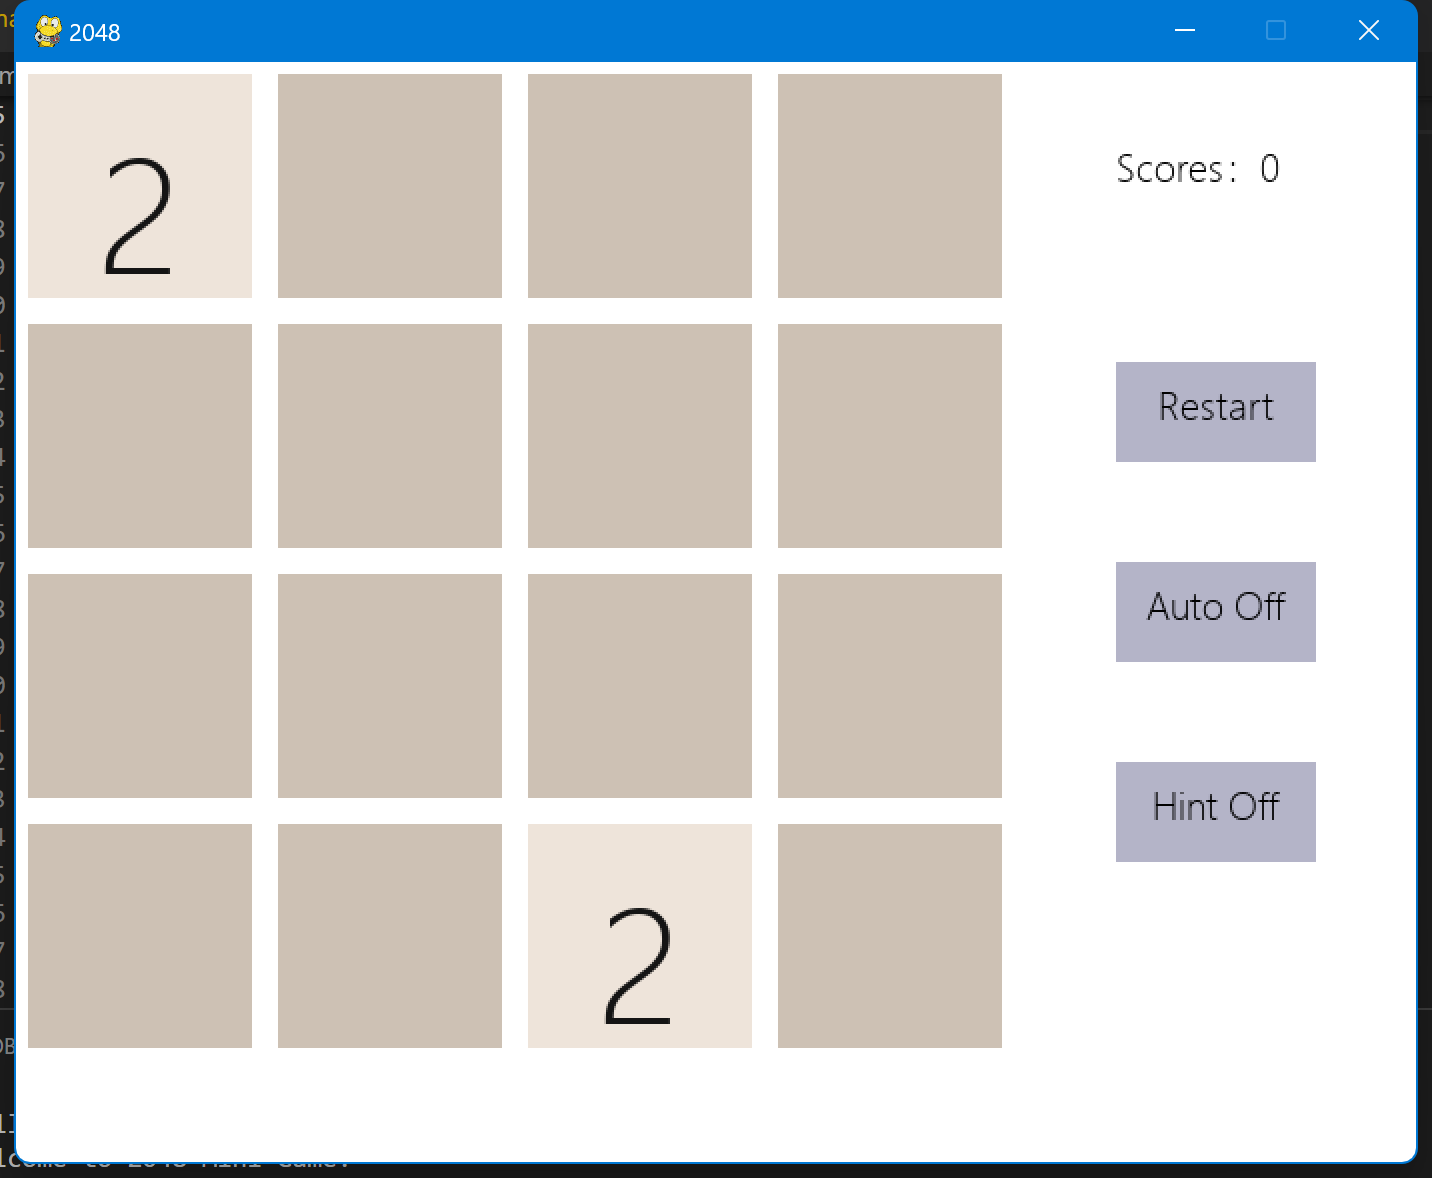
\includegraphics[width=0.7\linewidth]{img/pic1.png}
      \caption{示例图片}
      \label{fig:mergesort}
\end{figure}


\subsection{程序使用说明}
(详细描述如何使用你的程序,类似说明书)


\subsection{主要研究过程}
(详细描述你设计、调试程序的过程,类似开发日记)


\clearpage

\section{设计总结}

\subsection{成员分工}
(详细描述每位成员姓名、学号、班级、院系,以及分工完成的任务)

四位成员均来自电子信息学院A班,其分工信息如下表所示:

\begin{table}[!ht]
  \centering
  \caption{成员分工一览表}
  \label{tab:progress}
  \begin{tabular}{@{}cllc@{}}
    \toprule
    姓名 & \multicolumn{1}{c}{学号} & \multicolumn{1}{c}{分工}    \\ \midrule
    路人甲 & 2020301928          & 总体方案设计、撰写报告、维护GitHub项目、AI算法实现、验收答辩     \\
    路人乙 & 2020301923          & 游戏界面设计                   \\
    路人丙 & 2020301930          & 软件功能测试  \\ 
    路人丁 & 2020301927          & 方块移动模块的实现              \\ \bottomrule
  \end{tabular}
\end{table}

\subsection{存在的问题}
(详细描述你设计的程序仍然存在的问题)

\begin{itemize}
  \item 可以将游戏开始时的方块阶数集成至游戏界面中而不是终端,方便用户选择
  \item 可以适当添加一些游戏音效和动效,增强游戏的趣味性
\end{itemize}

\subsection{改进措施}
(对你设计的程序,未来可以从哪些具体地方使用什么措施进行改进)
\begin{itemize}
  \item 进一步学习用户界面设计,以期达到更好的用户体验
  \item 深入学习数据结构等相关知识,进一步优化当前算法,以期能够实现更加复杂的功能
\end{itemize}


\subsection{课程收获}
\begin{itemize}
  \item 路人甲
  \subitem 通过本课程的学习,我收获颇丰,受益匪浅。
  \item 路人乙
  \subitem 阿巴阿巴
 
\end{itemize}


\subsection{对课程的建议}
(每位成员谈谈对课程的设计、讲授等的建议)


\clearpage
\section{附录}
\subsection{程序源代码}

见电子压缩文档XXX.zip文件

(无需粘贴程序源码)


\subsection{其他}

若有其他附录文件,可写于此处,组织好格式

\subsection{致谢}

感谢老师一学期以来的指导与帮助。


\end{document}
